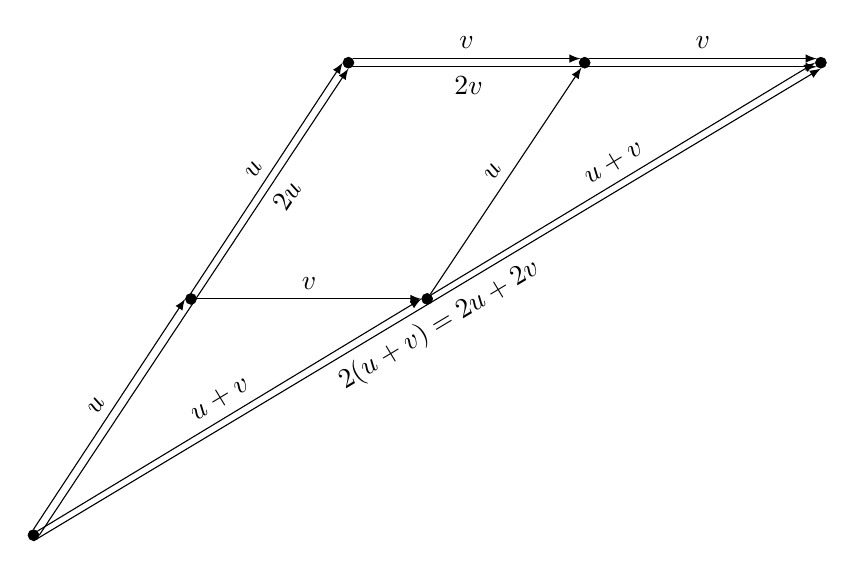
\begin{tikzpicture}[
	point/.style={circle,draw,very thin,fill,inner sep=0pt,minimum size=4pt},
	vector/.style={-latex},
]
	\node[point] at (0,0) (p) {};
	\node[point] at (2,3) (q) {};
	\node[point] at (4,6) (q2) {};
	\node[point] at (5,3) (r) {};
	\node[point] at (7,6) (s) {};
	\node[point] at (10,6) (r2) {};
	\draw[vector] (p.north) to node[above,sloped] {$\uvec{u}$} (q.west);
	\draw[vector] (q.north) to node[above,sloped] {$\uvec{u}$} (q2.west);
	\draw[vector] (p.east) to node[below,near end,sloped] {$2\uvec{u}$} (q2.south);
	\draw[vector] (q) to node[above] {$\uvec{v}$} (r);
	\draw[vector] (p.north east) to node[above,sloped] {$\uvec{u}+\uvec{v}$} (r.west);
	\draw[vector] (r.north east) to node[above,sloped] {$\uvec{u}+\uvec{v}$} (r2.west);
	\draw[vector] (q2.north east) to node[above] {$\uvec{v}$} (s.north west);
	\draw[vector] (s.north east) to node[above] {$\uvec{v}$} (r2.north west);
	\draw[vector] (q2.south east) to node[below,near start] {$2\uvec{v}$} (r2.south west);
	\draw[vector] (p.south) to node[below,sloped] {$2(\uvec{u}+\uvec{v}) = 2\uvec{u} + 2\uvec{v}$} (r2.south);
	\draw[vector] (r) to node[above,sloped] {$\uvec{u}$} (s);
\end{tikzpicture}
